\chapter{Catálogo de Segurança}
\label{chap:proposta}

Neste Capítulo, é apresentada uma primeira versão do catálogo de Segurança. Dado o volume de aspectos associados à Segurança, procurou-se focar nos aspectos mais relevantes, tomando como base a literatura. Portanto, o autor está ciente de que o catálogo proposto não acorda todo e qualquer aspecto associado à Segurança. Mas, a intenção do trabalho é apenas demonstrar que um catálogo construído para especificar RNFs, utilizando uma notação adequada, mesmo que em alto nível de abstração, pode colaborar no entendimento das necessidades inerentes aos aspectos não-funcionais de um software, comumente colocados em segundo plano, ou apenas especificados em documentos, em linguagem natural. Esses documentos, como a Especificação Suplementar \cite{sommerville1997requirements}, carecem de uma notação que permita especificar os RNFs com toda a complexidade envolvida, ou seja, partindo de  um alto nível de abstração, mas permitindo acordar operacionalizações, as quais de fato tornarão aquele RNF algo implementável, tratável a nível de código. Para a equipe de desenvolvedores, ter especificadas as operacionalizações, acorda soluções concretas para viabilizar a implementação de aspectos considerados tão abstratos. Para atingir esse objetivo, o catálogo proposto é especificado utilizando a notação do NFR \textit{Framework}, já comentada em capítulos anteriores. Essa notação propõe a elaboração de um grafo de interdependências entre os RNFs. Adicionalmente, deixa evidente as principais correlações entre esses RNFs, seus impactos e suas operacionalizações. Conforme justificado no Capítulo \ref{chap:introducao}, dada a relevância do RNF Segurança, têm-se que essa proposta foca seus esforços na especificação desse RNF.

Para tornar mais compreensível o catálogo, optou-se por apresentá-lo em dois níveis de detalhamento. Portanto, na seção \ref{sub:primeiroNivel}, tem-se um primeiro nível de detalhamento. Nesse nível, são acordadas as metas flexíveis (representando os RNFs), seus impactos e suas operacionalizações. Utilizou-se a notação do NFR \textit{Framework}, com a elaboração de um grafo, SIG (\textit{Softgoal Interdependence Graph}). Na seção \ref{sub:segundoNivel}, é apresentado um mapeamento, procurando correlacionar as metas flexíveis e as camadas do Padrão Arquitetural MVC. Um terceiro nível de detalhamento também é almejado nessa pesquisa, sendo esse o mapeamento entre as operacionalizações e as camadas do Padrão Arquitetural MVC. Entretanto, optou-se por construir esse último mapeamento, juntamente com o andamento do TCC 02, pois acredita-se que essa construção - por envolver aspectos em um nível mais baixo de abstração (implementando de fato as operacionalizações nas camadas \textit{Model-View-Controller}) - se tornará mais concreta com um software sendo desenvolvido. Portanto, a construção desse nível de detalhamento ocorrerá de forma dinâmica e evolutiva, ao longo do TCC 02.

\section{O Catálogo de Segurança}

Essa primeira versão do catálogo de Segurança procura promover aos engenheiros de requisitos e engenheiros de software uma maior compreensão quanto às diferentes necessidades em se tratando de Segurança. O catálogo acorda os principais conceitos associados à Segurança, tomando como base o levantamento bibliográfico realizado nessa pesquisa.

Conforme colocado anteriormente, o catálogo será apresentado em dois níveis de detalhamento. O primeiro nível, seção \ref{sub:primeiroNivel}, procura apresentar as metas flexíveis - ou RNFs - associadas à Segurança. O grafo especifica ainda as correlações e os impactos entre essas metas flexíveis bem como as operacionalizações (no nível mais baixo do grafo). O segundo nível é apresentado na seção \ref{sub:segundoNivel}, como um mapeamento entre as metas flexíveis e as camadas do Padrão Arquitetural MVC.

\subsection{Primeiro Nível de Detalhamento}
\label{sub:primeiroNivel}

O primeiro nível de detalhamento apresenta as metas flexíveis mais genéricas de Segurança de software, apoiando-se principalmente na definição de Chung. Essa definição baseia-se em Confidencialidade, Integridade e Disponibilidade. Adicionalmente, esse detalhamento também se apoia na definição de Segurança da Informação apresentada na ISO 27001. 

\begin{citacao}
	"Segurança da informação: preservação da \textbf{confidencialidade}, \textbf{integridade} e \textbf{disponibilidade} da informação; adicionalmente, outras propriedades, tais como \textbf{autenticidade}, \textbf{responsabilidade}, não repúdio e \textbf{confiabilidade}, podem também estar envolvidas." \cite[p. 2]{documentation2005information}
\end{citacao}


As metas flexíveis foram definidas de acordo com sua relação com Segurança. Observa-se que foram acrescentados, à notação do SIG, alguns valores, representados como referências. A intenção é permitir a rastreabilidade de cada aspecto representado no grafo com sua respectiva fonte ou referência teórica. Esse rastreamento permite - ao leitor: (i) ter a comprovação de que a especificação do catálogo foi de fato apoiada na literatura, e (ii) aprofundar seus conhecimentos - caso assim o desejar - consultando as referência para maior esclarecimento sobre cada especificação sugerida no catálogo. A Tabela \ref{indicesDeReferencia} apresenta os identificadores para a rastreabilidade da referência teórica de uma meta flexível no SIG da Figura \ref{DetalhamentoPrimeiroNivel}. 

\pagebreak

\begin{table}[h!]
	\centering
	\caption{Índices de rastreabilidade.}
	\label{indicesDeReferencia}
	\begin{tabular}{@{}cc@{}}
		\toprule
		\textbf{Identificador} & \textbf{Referência} \\ \midrule
		{[}1{]} & \cite{chung2012non} \\ 
		{[}2{]} & \cite{benitti2015taxonomia} \\
		{[}3{]} & \cite{documentation2005information} \\
		{[}4{]} & \cite{affleck2012supporting} \\
		{[}5{]} & \cite{buschmann1996system}
		\\ \bottomrule
	\end{tabular}
\end{table} 


\begin{figure}[h!]
	\centering
	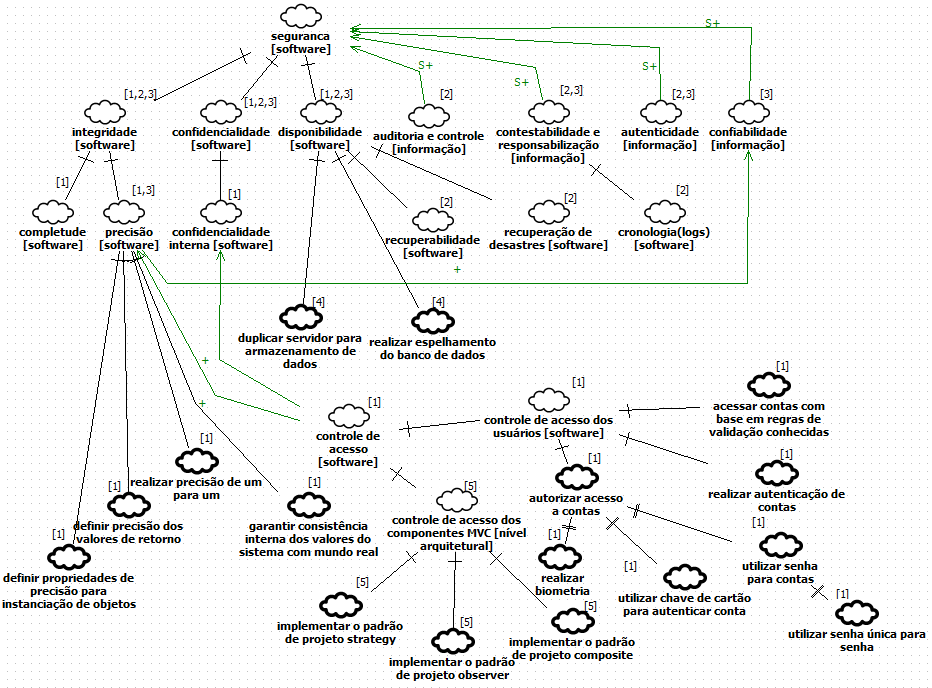
\includegraphics[keepaspectratio=true,scale=0.7]{figuras/CatalogoDeSeguranca.JPG}
	\caption{Catálogo de Segurança.}
	\label{DetalhamentoPrimeiroNivel}
\end{figure}


As definições das metas flexíveis são: 

\begin{itemize}
	
	\item \textbf{integridade:} Proteção contra qualquer tipo de atualização e/ou adulteração não autorizada. Definida na seção \ref{sec:seguranca}.
	
	\begin{itemize}
		
		\item \textbf{precisão:} Pode ser entendida como qualquer atributo semântico que fundamenta uma informação. Definida na seção \ref{sec:seguranca}.
		
		\begin{itemize}
			
			\item \textbf{\textit{definir propriedades de precisão para instanciação de objetos:}} Garantir que objetos sejam instanciados da maneira correta. Definida na seção \ref{sec:seguranca}.
			
			\item \textbf{\textit{definir precisão dos valores de retorno:}} Garantir que os valores retornados pelas operações possuem a precisão pré-estabelecida. Definida na seção \ref{sec:seguranca}.
			
			\item \textbf{\textit{realizar precisão de um para um:}} Garantir que um único objeto esteja ligado a uma única entidade do domínio. Definida na seção \ref{sec:seguranca}.
			
			\item \textbf{\textit{garantir consistência interna dos valores do sistema com mundo real:}} Garantir que os valores do mundo real sejam correspondentes aos valores do sistema. Definida na seção \ref{sec:seguranca}.
			
			\item \textbf{controle de acesso:} Nível mais genérico para autorização de acesso definido por \cite{chung2012non}, trata-se das especificações de controle de acesso do software. 
			
			\begin{itemize}
				
				\item \textbf{controle de acesso dos usuários:} Controle de acesso de usuários no software \cite{chung2012non}. Para ser satisfeita, depende de um conjunto de operacionalizações: \textbf{\textit{autorizar acesso a contas}}, \textbf{\textit{acessar contas com base em regras de validação conhecidas}} e \textbf{\textit{realizar autenticação de contas}}.
				
				\item \textbf{controle de acesso dos componentes MVC:} Trata-se das restrições arquiteturais impostas pelo padrão arquitetural MVC para que as relações internas entre os componentes sejam realizadas \cite{buschmann1996system}. Para que isso ocorra, devem ser implementados três \textit{design patterns}, que são abstraídos no catálogo de Segurança como operacionalizações, sendo elas: (i) \textbf{\textit{implementar o padrão de projeto strategy}}, \textbf{\textit{implementar o padrão de projeto observer}} e \textbf{\textit{implementar o padrão de projeto composite}}.
				
			\end{itemize}
						
		\end{itemize}
		
		\item \textbf{completude:} Garantia que o RNF esteja o mais completo possível. Definida na seção \ref{sec:seguranca}.
	\end{itemize}
	
	\item \textbf{confidencialidade:} Proteção da informação para evitar que as informações armazenadas ou transmitidas não sejam vistas ou interpretadas por terceiros, sendo somente o usuário principal e o destinatário. Definida na seção \ref{sec:seguranca}.
	
	\begin{itemize}
		
		\item \textbf{confidencialidade interna:} Proteção da informação que o acesso deve ser evitado por um público externo. Definida na seção \ref{sec:seguranca}.
		
	\end{itemize}
	 
	 \item \textbf{disponibilidade:} Proteção contra a interrupção do serviço, no momento em que o usuário estiver utilizando a aplicação. Definida na seção \ref{sec:seguranca}.
	 
	 \begin{itemize}
	 		
	 		\item \textbf{recuperabilidade:} Intervalo de tempo que o software deverá estar disponível após uma falha \cite{benitti2015taxonomia}.
	 	
	 		\item \textbf{recuperação de desastres:} Políticas e procedimentos aplicados na recuperação de ``desastres`` induzidos no software por usuário ou softwares de terceiros \cite{benitti2015taxonomia}.
	 		
	 		\item \textbf{\textit{duplicar servidor para armazenamento de dados:}} Promove menor chance de tempo onde ocorra a inatividade dos dados. Com a utilização de dois ou mais servidores em funcionamento, a disponibilidade dos dados do software é maior \cite{date2004introduccao}\cite{affleck2012supporting}.   
	 		
	 		\item \textbf{\textit{realizar espelhamento do banco de dados:}} Compreende-se como duas cópias de um único banco de dados que geralmente reside em máquinas diferentes \cite{date2004introduccao}\cite{affleck2012supporting}. 
	 		
	 \end{itemize}
 
 	\item \textbf{auditoria e controle:} Especificação dos aspectos que devem ser contemplados para proporcionar a auditoria e o controle \cite{benitti2015taxonomia}. 
 	
 	\item  \textbf{contestabilidade e responsabilização:} Capacidade do software em quantificar as ações e os eventos, com intuito de comprovar sua ocorrência \cite{benitti2015taxonomia}. 
 	
 	\begin{itemize}
 		
 		\item \textbf{cronologia(logs):} Registro de alterações no software \cite{benitti2015taxonomia}.
 		
 	\end{itemize}
 	
 	\item \textbf{autenticidade:} Pode ser entendida como a capacidade do software em identificar que um objeto ou recurso é o que ele realmente declara ser \cite{benitti2015taxonomia}. 
 	
 	\item \textbf{confiabilidade:} Pode ser entendida como a capacidade do software em realizar e manter seu funcionamento quando submetido em circunstâncias de rotina \cite{benitti2015taxonomia}. 
 	
\end{itemize}

\subsection{Segundo Nível de Detalhamento}
\label{sub:segundoNivel}

O segundo nível de detalhamento procura correlacionar as metas flexíveis mais genéricas e as camadas do Padrão Arquitetural MVC. As Tabelas \ref{mapeamento1} e \ref{mapeamento2} apresenta esse mapeamento, considerando diferentes níveis de satisfação para cada meta flexível.


Conforme comentado na introdução desse capítulo, pretende-se ter mais um nível de detalhamento na apresentação do catálogo proposto. Nesse nível, será possível correlacionar/mapear as operacionalizações e as camadas do Padrão Arquitetural MVC. Portanto, o conteúdo das Tabelas \ref{mapeamento1} e \ref{mapeamento2} poderá - sendo muito provável que ocorra - evoluir continuamente, junto ao andamento do TCC2. Acredita-se que ao desenvolver um software, com base no catálogo proposto até o momento, será possível compreender mais facilmente as correlações entre metas flexíveis, operacionalizações e camadas do Padrão Arquitetural MVC, permitindo refinar ainda mais o próprio catálogo (seção \ref{sub:primeiroNivel}) e seus níveis de mapeamento (seção \ref{sub:segundoNivel}) bem como ampliar as contribuições desse trabalho.

\begin{table}[h!]
	\centering
	\caption{Mapeamento das metas flexíveis com as camadas do MVC - Parte 1.}
	\label{mapeamento1}
	\tiny
	\begin{tabular}{@{}cccp{5cm}cc@{}}
		\toprule
		\multicolumn{1}{l}{\textbf{id}} & \multicolumn{1}{l}{\textbf{Meta flexível}} & \multicolumn{1}{l}{\textbf{\begin{tabular}[c]{@{}l@{}}Nível de\\ satisfação\end{tabular}}} & \multicolumn{1}{l}{\textbf{Descrição}} & \multicolumn{1}{l}{\textbf{Referência}} & \multicolumn{1}{l}{\textbf{Camada}} \\ \midrule
		1 & \begin{tabular}[c]{@{}c@{}}``precisão\\ {[}software{]}``\end{tabular} & Satisfeita & Se razoavelmente satisfeita, garante garante que um único objeto esteja ligado a somente uma única entidade do domínio. A model representa os aspectos do domínio da aplicação. - Atributo de precisão: precisão de um para um. & \begin{tabular}[c]{@{}c@{}}\cite{chung2012non}\\ \cite{buschmann1996system}\end{tabular} & \textit{Model} \\
		\rowcolor[HTML]{C0C0C0} 
		2 & \begin{tabular}[c]{@{}c@{}}``precisão\\ {[}software{]}``\end{tabular} & \begin{tabular}[c]{@{}c@{}}Satisfeita\\ Suficientemente\end{tabular} & Se razoavelmente satisfeita, garante que os objetos estejam sendo instanciados da maneira correta dentro da model. -Atributo de precisão: Propriedade da precisão & \begin{tabular}[c]{@{}c@{}}\cite{chung2012non}\\ \cite{buschmann1996system}\end{tabular} & \textit{Model} \\
		3 & \begin{tabular}[c]{@{}c@{}}``autenticidade\\ {[}software{]}``\end{tabular} & \begin{tabular}[c]{@{}c@{}}Satisfeita\\ Suficientemente\end{tabular} & A utilização de triggers em banco de dados promove a autenticidade e a verificação da integridade do dado, também pode ser utilizada para  realização de auditoria em tabelas. &  &  \\
		\cellcolor[HTML]{C0C0C0}4 & \cellcolor[HTML]{C0C0C0}\begin{tabular}[c]{@{}c@{}}``ìntegridade\\ {[}software{]}``\end{tabular} & \cellcolor[HTML]{C0C0C0}\begin{tabular}[c]{@{}c@{}}Satisfeita\\ Suficientemente\end{tabular} & \cellcolor[HTML]{FFFFFF} &  &  \\
		5 & \begin{tabular}[c]{@{}c@{}}``auditoria e\\  controle\\ {[}software{]}``\end{tabular} & \begin{tabular}[c]{@{}c@{}}Satisfeita\\ Suficientemente\end{tabular} & \multicolumn{1}{l}{} & \multirow{-3}{*}{\cite{date2004introduccao}} & \multirow{-3}{*}{\begin{tabular}[c]{@{}c@{}}Banco \\ de Dados\end{tabular}} \\
		\rowcolor[HTML]{C0C0C0} 
		\multicolumn{1}{l}{\cellcolor[HTML]{C0C0C0}6} & \begin{tabular}[c]{@{}c@{}}``controle\\  de acesso usuário\\ {[}software{]}``\end{tabular} & \begin{tabular}[c]{@{}c@{}}Parcialmente\\ Satisfeita\end{tabular} & O método de autenticação dos dados retorna a instância usuário, quando a senha está correta. Esse aspecto é implementado diretamente na \textit{Controller}. Entretanto, possui clara relação com a \textit{View} e com a base de dados. Considera-se "parcialmente satisfeita", pois há dependência com a operacionalização "Autorizar Acesso a Contas", a qual contribui para a satisfação dessa meta flexível "controle de acesso {[}software{]}". & \cite{fuentes2014ruby} & \textit{Controller} \\
		\multicolumn{1}{l}{7} & \begin{tabular}[c]{@{}c@{}}``confiabilidade\\ {[}informação{]}``\end{tabular} & Satisfeita & Se razoavelmente satisfeita, garante que o conjunto de dados a serem armazenados na base de dados estejam relativamente fidedignos. Usa-se "relativamente", pois não há como garantir algo pleno em se tratando de critérios tão abstratos. Nesse caso, "relativamente" sugere que seja "o mais fidedigno/confiável possível". & \cite{fuentes2014ruby} & \textit{View} \\ \bottomrule
	\end{tabular}
\end{table}

\begin{table}[p]
	\centering
	\caption{Mapeamento das metas flexíveis com as camadas do MVC - Parte 2.}
	\label{mapeamento2}
	\tiny
	\begin{tabular}{@{}cccp{5cm}cc@{}}
		\hline
		\multicolumn{1}{l}{\textbf{id}} & \multicolumn{1}{l}{\textbf{Meta flexível}} & \multicolumn{1}{l}{\textbf{\begin{tabular}[c]{@{}l@{}}Nível de\\ satisfação\end{tabular}}} & \multicolumn{1}{l}{\textbf{Descrição}} & \multicolumn{1}{l}{\textbf{Referência}} & \multicolumn{1}{l}{\textbf{Camada}} \\ \hline
		\rowcolor[HTML]{C0C0C0} 
		8 & \begin{tabular}[c]{@{}c@{}}``controle de \\ acesso dos \\ componentes \\ MVC\\ {[}nível arquitetural{]}``\end{tabular} & \begin{tabular}[c]{@{}c@{}}parcialmente\\ satisfeita\end{tabular} & Se parcialmente satisfeita, tende a garantir que os componentes da \textit{View}, os quais dependem de outros componentes que se encontram em outras camadas do modelo MVC, reconheçam a necessidade de atualizar as telas, adequando-as às demandas encaminhadas via \textit{Controller} (por exemplo) e em compatibilidade com os dados especificados na \textit{Model}. Considera-se "parcialmente satisfeita", pois há dependência com a implementação do padrão de projeto estrutural \textit{Composite}. A implementação é sugerida como operacionalização que contribue para satisfação dessa meta flexível, "controle de acesso dos componentes MVC {[}nível arquitetural{]}" & \begin{tabular}[c]{@{}c@{}}\cite{baptistella2011abordando} \\ \cite{buschmann1996system}\end{tabular} & \textit{View} \\
		9 & \begin{tabular}[c]{@{}c@{}}``controle de\\ acesso dos \\ componentes\\ MVC\\ {[}nível arquitetural{]}``\end{tabular} & \begin{tabular}[c]{@{}c@{}}parcialmente\\ satisfeita\end{tabular} & Se parcialmente satisfeita, tende a garantir que a \textit{Model} esteja menos acoplada em relação à \textit{View} e à \textit{Controller}, viabilizando essa relação através de boas práticas da Engenharia de Software. Uma dessas práticas é sugerida como operacionalização na Figura \ref{DetalhamentoPrimeiroNivel}, apoiando-se no uso de Padrões de Projeto. Considera-se parcialmente satisfeita, pois há dependência com a implementação do padrão de projeto comportamental \textit{Observer}, por exemplo. Essa implementação é sugerida como uma operacionalização possível em atendimento a essa demanda, e contribui para a satisfação dessa meta flexível, "controle de acesso dos componentes MVC{[}nível arquitetural{]}". & \begin{tabular}[c]{@{}c@{}}\cite{baptistella2011abordando} \\ \cite{buschmann1996system}\end{tabular} & \textit{Model} \\
		\rowcolor[HTML]{C0C0C0} 
		10 & \begin{tabular}[c]{@{}c@{}}``controle de\\ acesso dos \\ componentes\\ MVC\\ {[}nível arquitetural{]}``\end{tabular} & \begin{tabular}[c]{@{}c@{}}parcialmente\\ satisfeita\end{tabular} & Se parcialmente satisfeita, tende a garantir menor acoplamento entre as camadas MVC. Sugere-se que tal aspecto seja apoiado no uso de Padrões de Projeto. Portanto, acredita-se que o padrão de projeto \textit{Strategy}, implementado na \textit{Controller}, permita menor acoplamento entre \textit{View} e \textit{Model}, sendo de fato responsabilidade da \textit{Controller} intermediar essa relação utilizando-se de decisões estratégicas. Vale ressaltar que com o uso desse padrão de projeto, tem-se que essas decisões podem ser tomadas em tempo de execução, alterando o comportamento do software em função das demandas conhecidas dinamicamente. Dessa forma, há tendência é de maior cumprimento de boas práticas já acordadas no padrão arquitetural MVC. Considera-se parcialmente satisfeita, pois há dependência com a implementação do padrão de projeto comportamental \textit{Strategy}, por exemplo. Essa implementação é sugerida como uma operacionalização possível em atendimento a essa demanda, e contribui para a satisfação dessa meta flexível, "controle de acesso dos componentes MVC{[}nível arquitetural{]}". & \begin{tabular}[c]{@{}c@{}}\cite{baptistella2011abordando} \\ \cite{buschmann1996system}\end{tabular} & \textit{Controller} \\ \hline
	\end{tabular}
\end{table}

\pagebreak

\section{Resumo do Capítulo}

Neste capítulo, foi apresentada uma primeira versão do catálogo de Segurança, proposto nessa pesquisa. Adicionalmente, procurou-se acordar os principais impactos e as contribuições das informações do catálogo em relação às camadas do Padrão Arquitetural MVC. Ressalta-se que o catálogo foi especificado apoiando-se na literatura, conforme pode ser observado tomando como base a rastreabilidade apresentada na seção \ref{sub:primeiroNivel}.
Dada a complexidade do tema, em especial por procurar contribuir partindo de critérios de qualidade que são intrinsecamente abstratos e subjetivos, sabe-se que o catálogo ainda reflete uma visão preliminar sobre Segurança. Entretanto, acredita-se que a principal contribuição desse trabalho esteja sendo atendida, uma vez que vislumbra uma forma de trabalhar critérios tão abstratos (os requisitos não funcionais ou metas flexíveis e suas dependências e seus impactos), trazendo-os para uma visão bem mais concreta, as operacionalizações. Tudo garantido com o uso de uma notação bastante rica e emergente, a qual é muito mais conhecida e compreendida na subárea de Engenharia de Requisitos. Esse trabalho procura aproximar esse conhecimento, considerando um detalhamento mais técnico, para que outras atividades da Engenharia de Software (ex. Arquitetura e Desenho de Software e Desenvolvimento de Software) usufruam dessas contribuições. Assim, são apresentados detalhamentos que deixam evidentes as correlações entre esses níveis de abstração, Requisitos Não-Funcionais e Código, os quais parecem distantes. Essa distância comumente reflete em esquecimento, ou seja, não atendimento desses critérios de qualidade no desenvolvimento do software desejado. Prática essa que pode levar a muitos insucessos, tais como o Caso da Ambulância de Londres \cite{finkelstein1996comedy}.


Por fim, cabe mencionar que o catálogo ainda terá mais um nível de detalhamento, o qual irá focar em apresentar a correlação entre as operacionalizações e as camadas MVC. Esse nível será mais bem compreendido ao realizar o desenvolvimento de uma aplicação Web, tarefa a ser desempenhada ao longo do TCC2. Portanto, o catálogo evoluirá em alguns aspectos, o que permitirá que o mesmo contribua ainda mais em apresentar como critérios de qualidade podem ser suficientemente tratados e satisfeitos no nível de código.
